\documentclass{IEEEtran}

\usepackage{cite}
\usepackage{amsmath}
\usepackage{amssymb}
\usepackage{url}
\usepackage{graphicx}
\usepackage{booktabs}
\usepackage{microtype}
\usepackage[table]{xcolor}
\usepackage{tikz}
\usetikzlibrary{positioning,arrows.meta}
\usepackage[hidelinks]{hyperref}

\title{A Fairness-Aware Sequential Decision Framework for Clinical Diagnostic Workflows and Quantum Routing\\[0.3em]
{\large\textit{Comparing Multi-Armed, Contextual, and Informative Bandit Methods}}}

\author{%
\begin{minipage}{0.48\textwidth}
\begin{center}
{\bf Piter Z. Garcia}\\
\begin{small}
MS Data Science / Decision-Making \& Algorithmic Fairness\\
Rochester Institute of Technology (RIT)\\
{\it pizg8794@g.rit.edu}
\end{small}
\end{center}
\end{minipage}
\hfill
\begin{minipage}{0.48\textwidth}
\begin{center}
{\bf Dr. Daniel Krutz, Travis Desell}\\
\begin{small}
Department of Software Engineering, Data Science\\
RIT Research Advisors\\
{\it dxkvse@g.rit.edu, tjdvse@g.rit.edu}
\end{small}
\end{center}
\end{minipage}%
}

\begin{document}
\maketitle

\section{Approach Overview}
This work proposes a shared fairness-aware sequential decision framework for two domain-distinct but structurally similar settings: clinical diagnostic workflows and quantum-network routing/resource allocation. In both settings, a policy repeatedly selects actions under uncertainty from incomplete or unequal information, receives only partial feedback, and can accumulate group-dependent disparities over time. The main research target is therefore not simply whether bandit-based policies improve average utility, but whether uneven context quality, partial feedback, and shift create or amplify unfair outcomes during learning.

The method family is intentionally organized as a comparison spectrum rather than a single chosen algorithm. Multi-armed bandits provide a low-information baseline, contextual bandits test whether observed side information improves decisions, and informative-context methods test settings in which richer context is available but still noisy, delayed, or uneven across groups. This spectrum makes it possible to study whether additional context improves fairness, merely relocates disparities, or still requires explicit mitigation.

The two domains are studied together because they share one interaction logic while preserving different operational meanings. In the clinical setting, the sequential workflow includes decisions such as screening, confirmatory testing, and follow-up escalation, where weaker observed context for some patient groups may contribute to false-negative gaps or delayed intervention. In the quantum setting, the workflow includes route selection and scarce resource allocation under probabilistic link success and changing network conditions, where unfairness appears as persistent disparities in success rate, latency, or access across flow groups. The contribution is therefore a shared evaluation framework for fairness-aware sequential decision-making, not a loose pairing of two unrelated applications.

\section{Domain Model and Interaction Logic}
Figure~\ref{fig:domain_model} shows the shared domain model used across both testbeds. Each environment produces a decision state, exposes only the context available at that time, and may degrade that context through missingness, delay, noise, or group-dependent information quality. A policy from the selected method family then chooses an action, the environment returns partial feedback and reward, and the system logs both utility and fairness metrics over time. A mitigation and comparison loop uses those logged results to compare baseline and fairness-aware variants under the same experimental conditions.

\begin{figure*}[!t]
\centering
\resizebox{0.97\textwidth}{!}{%
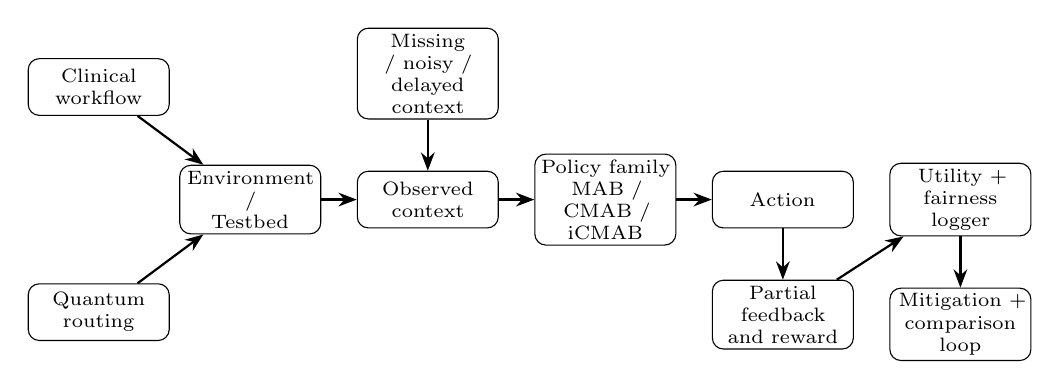
\begin{tikzpicture}[
font=\scriptsize,
box/.style={draw, rounded corners=4pt, align=center, text width=1.65cm, minimum height=0.72cm, inner sep=2pt},
arr/.style={-Stealth, thick}
]
\node[box] (env) {Environment /\\Testbed};
\node[box, above left=0.62cm and 0.12cm of env] (clin) {Clinical\\workflow};
\node[box, below left=0.62cm and 0.12cm of env] (quant) {Quantum\\routing};
\node[box, right=0.45cm of env] (ctx) {Observed\\context};
\node[box, above=0.65cm of ctx] (deg) {Missing / noisy /\\delayed context};
\node[box, right=0.45cm of ctx] (pol) {Policy family\\MAB / CMAB / iCMAB};
\node[box, right=0.45cm of pol] (act) {Action};
\node[box, below=0.65cm of act] (fb) {Partial feedback\\and reward};
\node[box, right=0.45cm of act] (log) {Utility + fairness\\logger};
\node[box, below=0.65cm of log] (mit) {Mitigation +\\comparison loop};

\draw[arr] (clin) -- (env);
\draw[arr] (quant) -- (env);
\draw[arr] (env) -- (ctx);
\draw[arr] (deg) -- (ctx);
\draw[arr] (ctx) -- (pol);
\draw[arr] (pol) -- (act);
\draw[arr] (act) -- (fb);
\draw[arr] (fb) -- (log);
\draw[arr] (log) -- (mit);
\end{tikzpicture}%
}
\caption{Shared domain model for the two testbeds. Both settings use the same fairness-aware sequential decision architecture while retaining different operational meanings and fairness metrics.}
\label{fig:domain_model}
\end{figure*}

This model justifies treating the domains as one methodology with two case-study branches. The common entities remain the same across both settings: environment/testbed, observed context, degraded-context mechanism, policy family, action, feedback, and fairness-aware logging. What changes is the domain-specific meaning of each entity. In the clinical branch, an action may be a diagnostic test or escalation step and fairness may be measured through false-negative or delayed-escalation gaps. In the quantum branch, an action may be a route or allocation decision and fairness may be measured through service-equity gaps in success or latency. Keeping the interaction logic shared while allowing the metrics to remain domain-specific is what makes the framework both coherent and credible.

\section{Why This Design}
Several design decisions follow directly from the research question. First, the clinical testbed is simulation-first rather than dependent on sensitive patient records. This allows controlled experiments under missingness, noisy observations, delayed feedback, and subgroup-specific context degradation without creating a data-access bottleneck. Second, the quantum case study extends an existing routing and resource-allocation foundation rather than introducing a toy second domain, which gives the cross-domain comparison technical credibility instead of making it a superficial transfer claim.

Third, the approach compares non-contextual, contextual, and informative-context methods because the project is studying how the amount and quality of available information changes fairness and utility behavior. A contextual-only study would hide whether richer context truly improves disparity outcomes relative to lower-information baselines. A post-hoc fairness audit would also be insufficient because the key claim is that fairness must be measured during learning, under partial feedback, rather than only after the policy has converged. Finally, a single-domain study would be easier to implement but would not test whether the same fairness-aware sequential decision principles remain meaningful across technically different systems. The shared framework is stronger precisely because it evaluates one methodology across two distinct but structurally aligned environments.

\section{Implementation Plan}
The implementation follows from the domain model rather than from a disconnected task list. A clinical simulation environment will model sequential diagnostic decisions such as screening, retesting, and escalation under subgroup-specific differences in observed context quality. An existing quantum routing environment will be integrated as the second testbed for repeated path-selection and resource-allocation decisions under probabilistic link success, changing load, and limited quantum resources. Both environments will expose the same policy interface so that multi-armed, contextual, and informative-context bandit variants can be evaluated through one shared execution pipeline.

Reward design will capture domain-specific utility outcomes such as diagnostic accuracy, intervention cost, success probability, and latency. Fairness design will capture disparities that matter inside each setting, including clinical false-negative or delayed-escalation gaps and quantum service-equity gaps across flow groups. Per-step logging, fixed random seeds, explicit configuration files, and modular experiment runs will support reproducibility and direct comparison across policies. At least one fairness-aware mitigation mechanism will be evaluated inside the same framework so that the final analysis measures both baseline disparity formation and the effect of mitigation during learning.

\begin{thebibliography}{9}\setlength{\itemsep}{0em}
\bibitem{garcia2025equitable_bioinformatics}
Garcia, P. Z. Equitable Bioinformatics: Enhancing Diagnostic Decision-Making through {RNA}
and Biomarker Data. Course paper (ISTE 780 Phase 4), Rochester Institute of Technology,
2025.
\bibitem{garcia2026threat_aware_quantum_routing}
Garcia, P. Z. Threat-Aware Evaluation of Quantum Entanglement Routing and Qubit Allocation
via Hybrid Contextual Bandits. Unpublished manuscript (GA-Work internal draft), Rochester
Institute of Technology, 2026.
\end{thebibliography}

\end{document}
